\documentclass[]{article}

\usepackage{amsmath}  % AMS math package
\usepackage{amssymb}  % AMS symbol package
\usepackage{bm}       % bold math
\usepackage{graphicx} % Include figure files
\usepackage{dcolumn}  % Align table columns on decimal point
\usepackage{multirow} % Multirow/column tables
\usepackage{hyperref} % Hyperlinks

\begin{document}

\title{Modeling Ising}
\author{Scott O'Connor}
\date{\today} 
\maketitle

  \begin{abstract}
  The ising model is used in this program as a way to predict the behavior of magnetic material as it is effected by temperature. 
  \end{abstract}

\section{Program Explained}
  \subsection{}
  The first thing this model does is calculate the Hamiltonian.
  This is done by summing the states of each location in the Lattice
  \begin{equation}
      H(\sigma) = - \sum_{i=1} \sigma_i \sigma_j 
  \end{equation}
  For a 2D case there are four possible nearest neighbor interations: the cell above, below, left and right.
  The lattice currently implimented is zeropadded. This allows for the ability to sum over the non-zero padded portion of the lattice and not have to worry about the boundries. 

  After the intial calacluaiton of the hamiltonian, a monte carlo simulation is performed on the lattice. In the monte carlo routine, random bits are selected, and a metropolis test is performed
  The metropolis test will determined if a bit should be fliped or not.

  \begin{equation}
      \Delta E = 2 \sigma_i (\sigma_{above} + \sigma_{below} + \sigma_{left} \sigma_{right})
  \end{equation}

  \begin{equation}
    X \sim [(0,1)]< e^{-\beta \Delta E}
  \end{equation}
 

\section{Plots} 
 %Plotting normalized magnetization vs various temperatures, the magnetization goes to zero around 2.2. This is consistant with how the model should perform   
    \begin{figure}[b]
      \centering
      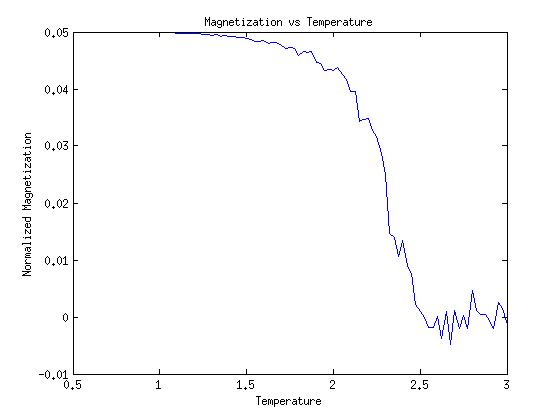
\includegraphics{figures/mag_vs_temp.jpg}
      \caption{\label{fig:mag_vs_temp}Normalize Magnetization and various temperatures}
    \end{figure}

 %Plotting the magnetization over a million iterations in a 100 by 100 lattice when the temperature is temp=1, results in a net magnetization. 
    
    \begin{figure}[b]
      \centering
      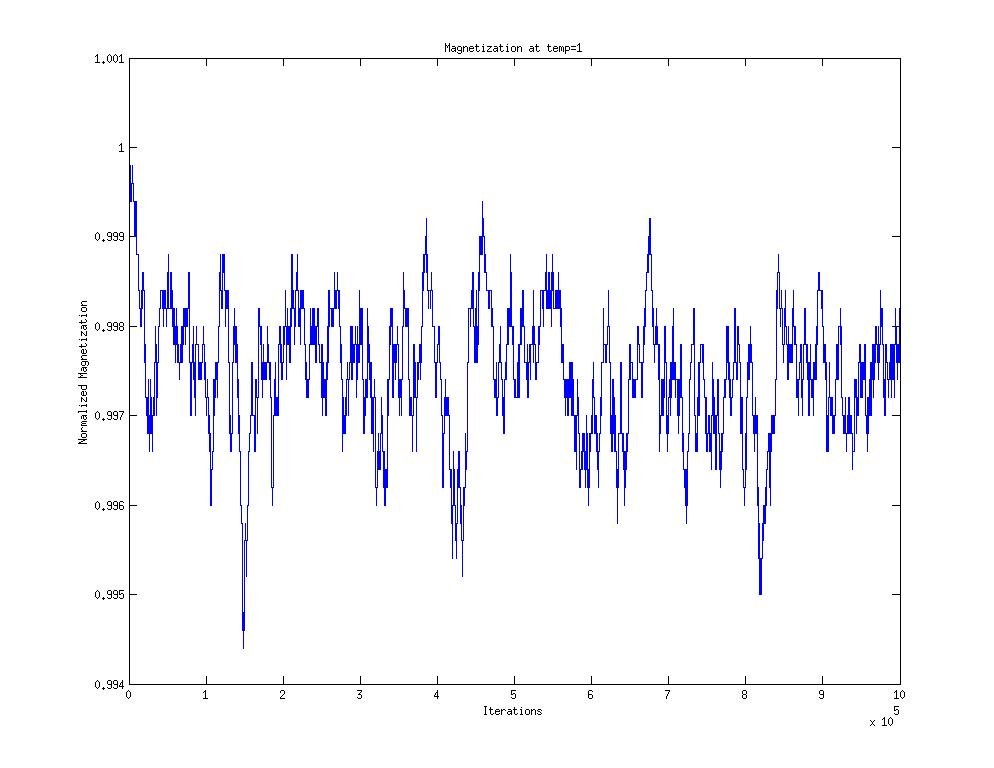
\includegraphics{figures/mag_t1.jpg}
      \caption{\label{fig:mag_T1p} Magnetization over a million iterations at temp=1}
    \end{figure}
    
%Plotting the same simulation as above, except that temp=3 results in a zero net magnetization.

    \begin{figure}[b]
      \centering
      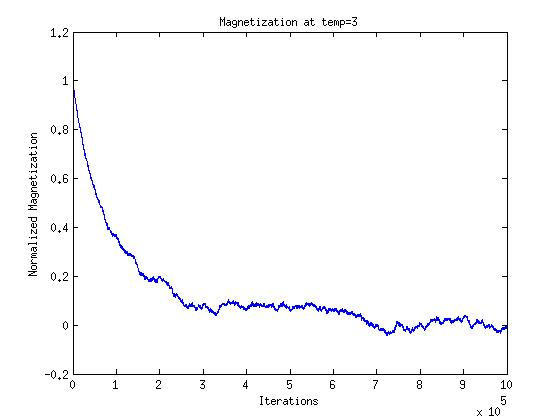
\includegraphics{figures/mag_t3.jpg}
      \caption{\label{fig:mag_T3p} Magnetization over a million iterations at temp=3}
    \end{figure}

\section{Energy at Different Temperatures}

    \subsection{\label{sec:level2} Temperature at 2}

    \subsection{\label{sec:level2} Temperature at 3}

\begin{conclusion}
The results of the ising model are as expected. The magnetization goes to zero when temp=2.2. When the temperature is below this mark, the magntization hovers above zero. When the temperature is above zero the net magnetization goes to zero. 
\end{conclusion}

\end{document}
